\documentclass[11pt]{article}
\usepackage[T1]{fontenc}
\usepackage[margin=1in]{geometry}
\usepackage{amsmath,amssymb,booktabs,longtable,microtype}
\usepackage{tikz,pgfplots}
\pgfplotsset{compat=1.17}
\usepackage[colorlinks=true,linkcolor=teal,citecolor=teal,urlcolor=teal]{hyperref}
\title{FlashNS: Operator- and Adjoint-Aware Contracted Derivative Execution for High-Order PINNs}
\author{Dezhen Lu\\University of Tübingen\\\texttt{dezhen.lu@student.uni-tuebingen.de}}
\date{Updated research draft: October 13, 2026}
\begin{document}\maketitle




\begin{abstract}
High-order physics-informed training requires coordinate derivatives and their complete parameter gradients. FlashNS executes consumer-specific derivative states with parameter transposes and bounded chunk workspaces. In the original two-dimensional FP64 Navier--Stokes experiment on NVIDIA H20, all 18 representation-study solves and all 54 matched public-comparison solves pass unchanged numerical and independent scalar-AD acceptance. The eight-channel GL8 implementation gives 1.659$\times$ paired setup-plus-optimization speedup over compiled compact Q10; the public collapsed Taylor, explicit differentiation and exact two-dimensional STDE adaptations give respective baseline/GL8 ratios of 1.730, 2.312 and 3.368. We extend the study to a three-dimensional transient curl-potential model with a 36-channel partial derivative state, 4,999 objective points and all 50,692 parameters. Full H100 objective-gradient checks pass the frozen numerical budget. A packed-gather candidate nevertheless remains slower than C36 Taylor-state parameter AD: paired baseline/candidate ratios are 0.973 in eager mode and 0.970 with CUDA Graph replay. A subsequent packed activation with analytic activation transpose gives 1.0446$\times$ paired H100 CUDA Graph speedup over parameter AD using the same packed forward (95\% interval 1.0441--1.0451). Compiling the packed forward in both GPU arms and the candidate activation transpose gives 1.3240$\times$ on H100 (interval 1.3231--1.3248); the corresponding one-thread CPU result is 1.265$\times$ (interval 1.203--1.328). Both H100 training engines complete their frozen two-seed budgets, but neither passes the prescribed convergence and physical acceptance criteria. The results establish the stated execution tradeoffs and numerical qualifications; they do not establish three-dimensional time-to-accuracy acceleration or a fluid regularity theorem.
\end{abstract}

\section{Introduction}
Training a physics-informed neural network (PINN) requires derivatives of a
network output with respect to coordinates and derivatives of the resulting
loss with respect to every network parameter. These are different consumers.
For gradient-enhanced incompressible Navier--Stokes training, the residual
uses second coordinate derivatives and its gradient uses third derivatives.
A fast residual evaluation does not establish a fast training step, and a
fast training step does not establish a shorter solve to a prescribed error.

Taylor-mode and explicit derivative methods already address the cost of
nested coordinate automatic differentiation (AD). Residual-specific partial
jets, collapsed Taylor propagation and stochastic Taylor contractions are
especially relevant to this problem~\cite{cao,cmtad,stdepp}. We build on that
setting. Our question is whether a concrete operator contraction, its
complete parameter transpose and a practical bounded working-state schedule
can improve an unchanged third-order training objective beyond a compiled
full-jet implementation and public derivative methods.

For this objective, independent third partials are not needed: the diffusion
consumer asks for the gradient of the Laplacian. We retain the scalar value,
coordinate gradient, symmetric Hessian and gradient of the Laplacian. In two
dimensions this is an eight-channel state, GL8, instead of the ten channels
of a complete third-order state, Q10. Closure through an activation includes
products between lower derivatives. Its parameter transpose additionally
depends on the fourth activation derivative. Omitting that dependence would
change the parameter gradient even if some forward residuals agreed.

FlashNS makes this consumer contract explicit and implements both sides of
it. It keeps matrix multiplications in library GEMMs, uses explicit CUDA
rules for pointwise derivative propagation and residual seeds, and replays
the complete loss/gradient computation with current parameter storage.
Boundary points use a value-only path. A chunked mode reuses one interior
workspace and accumulates the complete globally weighted parameter gradient
before any optimizer update.

We evaluate the implementation on the original FP64 Kovasznay
gradient-enhanced objective, including all six numerical acceptance criteria
and a separate scalar-AD final check. The representation study uses six
initialization seeds; the public comparison reuses those planned seeds and
reports its actual coverage. Paired comparisons use identical data and
initial parameter bytes. We
report full-gradient replay, setup, optimization and process wall time
separately. Public competing implementations are pinned and adapted to the
same objective; their adaptations and application limits are stated
explicitly. Development qualification never supplies a formal solve result.

The resulting contribution is a verified execution case study: a closed
contracted derivative state with its complete parameter VJP, a reusable
chunked implementation, and a source-pinned comparison of actual solves.
It does not establish the first residual-aware derivative method, a globally
minimal state, or superiority across PDEs, precisions or GPU families.


This revision preserves the October 6 H20 campaign and adds a separate
three-dimensional transient C36 study in Section~\ref{sec:c36}.
The two campaigns have different models, source data, parameter counts,
seeds, acceptance gates and hardware; their timings are never pooled.
The H20 comparisons remain accepted solve measurements. The new H100 and
CPU ratios measure complete objective/gradient evaluations, while the new
three-dimensional solver acceptance remains unsuccessful.

\section{Contracted derivative execution}
\subsection{A fixed scientific objective}
We study steady incompressible flow with constant viscosity $\nu$ and physical
Cartesian coordinates $x=(x_1,x_2)$. A neural network predicts $(u,v,p)$.
Its residual is
\begin{align}
r_u&=u u_{x_1}+v u_{x_2}+p_{x_1}-\nu\Delta u,\\
r_v&=u v_{x_1}+v v_{x_2}+p_{x_2}-\nu\Delta v,\\
r_d&=u_{x_1}+v_{x_2}.
\end{align}
Following the gradient-enhanced objective~\cite{gpinn}, we retain both the
residual and its coordinate gradient:
\begin{equation}
L=\tfrac12\operatorname{mean}_{\Omega}
\left(\|r\|_2^2+0.2\|\nabla r\|_F^2\right)
+5\left(\operatorname{mean}_{\partial\Omega}
\|(u,v)-(u_*,v_*)\|_2^2+
\operatorname{mean}_{x_1=1}(p-p_*)^2\right).
\end{equation}
This objective needs third coordinate derivatives. Removing the gradient
penalty would change the scientific problem. All implementations use the
existing point weights and validation definitions; in particular, the
boundary component RMS is not the training vector-square mean.

\subsection{A closed representation}
For a scalar intermediate $z$, define
\begin{equation}
S(z)=(z,g,H,t),\qquad g=\nabla z,\quad
H=\nabla^2 z,\quad t=\nabla\Delta z.
\end{equation}
Only independent symmetric Hessian entries are stored. In two dimensions
the raw, unnormalized state is
\begin{equation}
(z,z_{x_1},z_{x_2},z_{x_1x_1},z_{x_1x_2},z_{x_2x_2},
 z_{x_1x_1x_1}+z_{x_1x_2x_2},
 z_{x_1x_1x_2}+z_{x_2x_2x_2}).
\end{equation}
We call this state GL8. It has eight channels per hidden scalar, compared
with ten for the complete third-order two-dimensional Taylor state Q10.
The raw-to-Taylor projection includes the appropriate factorials; GL8
channels must not be read as Taylor coefficients.

For a pointwise activation $y=\phi(z)$, let $a_k=\phi^{(k)}(z)$. Direct
application of the chain rule gives
\begin{align}
g_y&=a_1g,\\
H_y&=a_1H+a_2gg^\top,\\
t_y&=a_1t+a_2\left(g\,\operatorname{tr}H+2Hg\right)
          +a_3g\|g\|_2^2.
\label{eq:closure}
\end{align}
An affine layer applies the same weight matrix to each state channel,
with the bias added only to the value channel. Consequently, affine
layers and smooth pointwise activations form a closed execution rule for
$S$. The state supplies every quantity in $r$ and $\nabla r$: convection
gradients need the Hessian, while diffusion gradients need $t$.

Closure is sufficient for this consumer, not a claim of global
minimality or a reconstruction of all third derivatives. For example,
$z=x_1^3-3x_1x_2^2$ has $S(z)=0$ at the origin but
$z_{x_1x_1x_1}=6$. A request for an independent third partial cannot be
answered from GL8. The runtime rejects unsupported coordinate identities
or contractions instead of returning such an observable.

\subsection{Complete parameter adjoints}
Reducing the forward state alone is insufficient for training. FlashNS
transposes the same local closed rules, including their dependence on
the primal value. To make that dependence explicit, define
$Q=g\operatorname{tr}H+2Hg$ and $c=g^\top g$. The differential of the
third contracted component is
\begin{align}
\delta t_y={}&a_1\delta t+
a_2\left(\delta g\,\operatorname{tr}H+
g\,\operatorname{tr}\delta H+2\delta H g+2H\delta g\right)\nonumber\\
&+a_3\left(c\,\delta g+2g(g^\top\delta g)\right)
+\left(a_2t+a_3Q+a_4gc\right)\delta z.
\label{eq:differential}
\end{align}
Thus the local reverse rule requires $a_4$, although the forward
coordinate state stops at order three. The value, gradient and Hessian
differentials are transposed together with~\eqref{eq:differential}.
For the packed symmetric Hessian, off-diagonal entries use the transpose
of symmetric unpacking: the two matrix contributions are added, not
treated as two independent stored channels.

If $X$ is a layer input state and $\bar Z$ its preactivation adjoint,
the complete parameter updates are
\begin{equation}
\bar W=\sum_{n,q}\bar Z_{nq}X_{nq}^{\top},
\qquad \bar b=\sum_n\bar Z_{n,0},\qquad
\bar X_{nq}=W^\top\bar Z_{nq}.
\end{equation}
The implementation uses flattened point/channel matrix multiplications
for these reductions. A fixed polynomial residual program seeds all nine
residual and residual-gradient terms. It is a specific, verified consumer
rule rather than a general symbolic residual compiler.

In exact arithmetic, projection of a complete coordinate jet commutes
with the closed affine/activation rules. Composing with a loss that
depends only on that projection therefore preserves its parameter
derivative by the ordinary chain rule. Our numerical checks test both
the projected forward quantities and the entire flattened parameter
gradient; forward agreement alone would not establish this property.

\subsection{Stable activation and bounded working state}
The production kernels reuse the existing stable $\tanh$ convention.
In particular, the first derivative is evaluated with a stable
exponential tail instead of relying exclusively on subtraction from a
rounded saturated value. Higher derivatives and their reverse rules use
the same primal convention. Affine work remains in library GEMMs;
pointwise activation and residual transposes use explicit CUDA kernels.
CUDA Graph replay reads the current parameter storage rather than a
snapshot, which is checked by consecutive in-place updates.

Dirichlet and outlet consumers that need only values use a separate
value-only path. The chunked implementation processes interior points
in blocks of 512 and accumulates the complete parameter gradient using
the original global weights. It never normalizes each chunk separately.
Its working-state bound is proportional to chunk size, while fixed data,
parameters and optimizer storage remain outside that bound. Floating
reduction order can alter line-search trajectories; every backend must
still satisfy the same independent final criteria.

The measured GL8 production scope is two-dimensional, constant-viscosity,
pointwise affine/$\tanh$ networks with first parameter VJPs. The current
contract does not support a learned contraction, nonlinear coordinate
changes, sample-coupled layers, nonlocal losses, HVPs or double backward.


\section{Relation to existing derivative methods}
Physics-informed networks put PDE constraints into a training
objective~\cite{pinn}; gradient-enhanced training also penalizes residual
derivatives~\cite{gpinn}. Our contribution concerns execution of that
unchanged derivative-intensive objective.

Cao et al.~\cite{cao} already exploit residual-dependent partial jets
and specialized layer rules, checking residuals and parameter gradients.
FlashNS therefore does not claim priority for propagating only
PDE-relevant derivative information. The comparison here examines a
specific contracted state together with an explicit complete parameter
transpose and bounded interior working storage.

Dangel et al.~\cite{cmtad} collapse derivative sums within Taylor-mode
computation for linear differential operators. This is closely related
to retaining contractions instead of a full tensor. We evaluate the
public collapsed transform, including parameter backward and the
additional residual-gradient consumer. Merely comparing with our own
older compiled full-jet implementation would not constitute this
external baseline.

STDE and its extension~\cite{stde,stdepp} use high-order Taylor
directions and contractions to avoid materializing large derivative
tensors. The JMLR code link currently points to the public STDE
repository. Our two-dimensional exact-coordinate adaptation evaluates
that code; it is neither a separate implementation of every STDE++
mixed-partial construction nor an experiment on high-dimensional
stochastic amortization. Those distinctions bound the comparison.

The baseline adapters and precise source commits are part of the
artifact. Their measured results pertain to the matched scientific
objective and execution modes, not to each method's full application
range or the speedups originally reported on other workloads.


\section{Experimental protocol}
\subsection{Problem, data and acceptance}
The analytic Kovasznay solution is
\begin{equation}
u_*=1-e^{\lambda x_1}\cos(2\pi x_2),\quad
v_*=\frac{\lambda}{2\pi}e^{\lambda x_1}\sin(2\pi x_2),\quad
p_*=\frac{1-e^{2\lambda x_1}}{2},\qquad
\lambda=\frac{1}{2\nu}-\sqrt{\frac{1}{4\nu^2}+4\pi^2}.
\end{equation}
We set $\nu=0.07$ on $[-0.5,1]\times[-0.5,1.5]$. The network has widths
$2$--$64$--$64$--$3$, two $\tanh$ hidden layers, a linear head and 4,547
parameters. Training uses 2,048 interior points and 128 points on each of
four edges. The 128 pressure-outlet points share the last edge's coordinates;
there are 512 boundary coordinates, not 640. We retain the original globally
normalized interior, velocity and outlet weights.

The fixed stop-check set contains 8,192 interior points and 257 points on
each boundary edge. A separate scalar nested-AD interior set verifies every
candidate final solution. Both validations must meet all six limits in
Table~\ref{tab:thresholds}, with finite values. PDE RMS combines the three
residuals by the original sum-of-squares convention. Boundary velocity RMS
averages velocity components, whereas the training loss uses their vector
square. We preserve these definitions rather than reconstructing them from
metric names. Five data/weight SHA256 values are identical across every
matched run; initialization affects parameters only.

\begin{table}[t]
\centering
\caption{Unchanged numerical acceptance limits. A run succeeds only if both
the fixed validation and independent scalar-AD validation satisfy every row.}
\label{tab:thresholds}
\begin{tabular}{lc}\toprule
Metric & Upper limit\\\midrule
Combined PDE residual RMS & 0.02\\
Boundary velocity component RMS & 0.01\\
Outlet pressure RMS & 0.01\\
Relative $L_2$ error of $u$ & 0.01\\
Relative $L_2$ error of $v$ & 0.02\\
Relative $L_2$ error of $p$ & 0.02\\\bottomrule
\end{tabular}
\end{table}

\subsection{Optimizer and finite attempts}
Every formal arm uses the same optimizer and stopping program. Adam permits
4,000 updates with learning rate $10^{-3}$, halved every 1,000 updates,
$\beta=(0.9,0.999)$ and $\epsilon=10^{-8}$. Stop checks occur before training
and every 100 Adam updates. Strong-Wolfe L-BFGS then permits at most 500
blocks, each with 20 iterations, nominal 25 evaluations, history size 50,
learning rate 1, gradient tolerance $10^{-12}$ and change tolerance
$10^{-15}$. Stop checks follow each block. Line searches may exceed a
nominal evaluation limit; reported closure counts are actual counts.

The two-dimensional formal seeds are 862101--862106. Its development
seeds 361901 and 361902 and older regression seeds are excluded from the
two-dimensional formal comparisons. The new three-dimensional campaign
uses its separately frozen original seeds 361901 and 361902. No seed,
threshold or optimizer budget is changed after an observed result. Every
attempt is retained. Nonconvergence consumes its measured cost and counts
against the attempted arm; an unsupported execution variant does not turn
into a successful baseline through substitution. Paired time ratios are
computed only when both members pass and are accompanied by all outcomes.

The Q10/GL8/chunk campaign balances the six permutations of three arms.
The subsequent public comparison has six paper-group arms; three sampled
permutations and their reverses balance their order over the same six seeds.
NVIDIA baselines use separately admitted windows, so their timings are not
interleaved with paper-group controls. This shared H20 runs one admitted GPU
window at a time. All recorded children finish naturally. Whole-window
ownership includes copying and checking evidence before explicit handback.

\subsection{Baselines and execution modes}
\textbf{Q10 compact} propagates the complete two-dimensional third-order
Taylor state at interior points and values at boundaries. It uses the
existing explicit parameter transpose, full-graph Torch compilation and
CUDA Graph replay. It is a strong internal representation control, not the
public collapsed Taylor package.

\textbf{Cao ED} calls the pinned author's \texttt{ed\_u\_jet} without changing
that function. Its value, first derivatives and diagonal second derivatives
assemble the Navier--Stokes residual. Coordinate AD of that residual adds
the original gradient-enhancement term; parameter AD supplies the complete
gradient. This is a matched-objective adaptation of the public implementation.
We also execute the unmodified original author NS training recipe separately;
its architecture, objective and timing are not pooled with matched solves.

\textbf{Collapsed Taylor} calls the public \texttt{jet(collapsed=True)}
transform with exact coordinate directions. The collapsed second-order
output supplies the Laplacian, and residual coordinate AD supplies the
additional third-order consumer. Parameter AD is included. We test both the
default complete loss/gradient program and its traced, compiled variant.

\textbf{STDE exact} calls the public \texttt{hess\_diag} sparse-STDE operator
with dimension two, \texttt{rand\_batch\_size=0} and no randomized Jacobian.
The two coordinate directions are exhausted, so this experiment uses no
stochastic derivative estimator. JAX forward residual differentiation and
parameter backward preserve the same loss. JAX runs on the GPU in FP64;
CPU fallback is rejected. DLPack exchange, copies and synchronization with
the common Torch optimizer are included in replay and solve wall time.
This experiment does not evaluate every STDE++ mixed-partial construction
or its intended high-dimensional stochastic setting.

\textbf{Torch AD} evaluates nested coordinate AD and complete parameter
backward on an ordinary dense MLP. \textbf{PhysicsNeMo}~\cite{physicsnemo} uses the public
\texttt{PhysicsInformer} with symbolic Navier--Stokes equations and its
autodiff gradient method, followed by residual-gradient AD and parameter
backward. It is the full residual path, not just a standalone gradient
component.

\textbf{cuDNN}~\cite{cudnn} uses an algebraically equivalent $1\times1$ convolution MLP
with coordinate and parameter AD. A cuDNN operator must appear in the actual
profiler trace; a fallback is retained as a failed qualification rather than
called a cuDNN result. \textbf{cuEquivariance polynomial}~\cite{cueq} reuses the inherited
FP64 Q10 segmented-polynomial forward and explicit parameter VJP with the
native \texttt{uniform\_1d} backend. That implementation retains its
unmodified all-points Q10 policy, including boundaries. Scalar-irreps
\texttt{Linear} fused-tensor-product variants are separate diagnostics and
cannot replace the polynomial formal arm. Actual native operators are
required in the profiler.

For Torch-based public adapters and exact STDE, high-order derivatives run
only at the 2,048 interior points and values only at 512 boundary points,
matching the Q10/GL8 controls' point policy. Public adapters use
\texttt{torch.tanh}, while production FlashNS preserves its stable tail
convention. Mathematically they represent the same activation; numerical
full-gradient equivalence is checked rather than assumed.

\subsection{Qualification, caches and timing scopes}
Qualification evaluates the complete loss and all 4,547 parameter gradients
against the full-jet reference after each of three consecutive in-place
updates. The unchanged numerical tolerance is absolute $2\times10^{-12}$
and relative $2\times10^{-11}$. It also checks actual native execution where
required. Passing default/compiled variants are selected by the smallest
development median complete-gradient wall time; the selection map and
report hashes are frozen before formal seeds. No failed variant is used.

Qualification warms task-owned Torch, native-extension, Triton and JAX
caches. Each formal attempt is a fresh process with new parameters,
optimizer state and graphs. Persistent JAX compilation caching is explicitly
enabled, with compile threshold zero and entry threshold $-1$; cache
settings and hit/miss logs are retained. The resulting solve experiment is
a warm-dependency execution comparison. Initial qualification/build cost
is reported separately and is not silently amortized over the six seeds.

Complete-gradient qualification uses five groups of 30 replays after a
two-second warm-up and reports the median group wall time. The earlier
representation/memory study instead uses five independently ordered
processes per shape/arm, each with seven groups of 100 replays; these are
separate experiments. Replay timing includes full loss, every parameter
gradient and chunk/interoperation costs, but excludes optimizer, stop
validation and setup.

Optimization wall time includes training, optimizer work, line searches,
synchronization, stop checks and independent final acceptance. Setup plus
optimization additionally includes per-run engine preparation. It excludes
interpreter startup, common data creation and teardown; full child-process
wall time includes those costs. We report paired geometric means of time
ratios, not ratios of unpaired medians. Small-sample ranges are descriptive,
not a general-PDE confidence guarantee.

The GPU is NVIDIA H20 (SM90, 97,871 MiB), driver 580.76.05, CUDA toolkit
13.0.88, Torch 2.12.1+cu130 and Triton 3.7.1. All matched experiments use FP64 and
TF32 is disabled. JAX is 0.11.2; the native cuEquivariance ops package is
0.12.0. New dependencies live in a task-owned environment inheriting the
unchanged base numerical stack. This original two-dimensional campaign reports H20 measurements only.
The separate H100 and CPU measurements added in this revision are described
in Section~\ref{sec:c36}; no new Blackwell, SM120 or multi-GPU result is claimed.


The representation, memory and profiler study used the earlier physical H20 \texttt{edf64e5f}; the current public comparison, with six planned seeds, uses physical H20 \texttt{d952768b}. All current public measurements use the latter device; the planned NVIDIA comparisons use that same device. Earlier public campaigns remain archived separately and are not pooled with the current public timing comparison. Pairwise ratios are computed within their own device-specific campaign.


\section{Two-dimensional H20 results}

\subsection{Complete-gradient qualification}

\begin{table}[t]
\centering\small
\setlength{\tabcolsep}{4pt}
\caption{Development GPU qualification on seed 361902. Median complete loss/all-parameter-gradient wall time from five groups of 30 replays; optimizer, validation and setup excluded. Each passing variant satisfies three successive updated-parameter checks. JAX exchange is included. A missing value indicates failed qualification, not zero time.}
\label{tab:qualification}
\begin{tabular}{llrr}\toprule
Method & Selected execution & Gradient ms & Max gradient error\\\midrule
FlashNS GL8 & Native + graph & 1.583 & $7.55\times10^{-15}$\\
Q10 compact & Inductor + graph & 3.267 & $3.55\times10^{-15}$\\
Collapsed Taylor & Compiled + graph & 3.751 & $5.33\times10^{-15}$\\
Cao ED & Compiled + graph & 5.725 & $5.33\times10^{-15}$\\
Torch coordinate AD & Compiled + graph & 7.651 & $5.33\times10^{-15}$\\
STDE exact (2D) & JAX JIT & 9.459 & $5.33\times10^{-15}$\\
PhysicsNeMo & Compiled + graph & 6.506 & $5.33\times10^{-15}$\\
cuDNN convolution AD & Compiled + graph & 74.004 & $5.33\times10^{-15}$\\
cuEquivariance polynomial & Native polynomial + graph & 3.340 & $5.33\times10^{-15}$\\
\bottomrule\end{tabular}
\end{table}


9 of 9 paper-group development variants pass the complete-gradient checks; their largest observed absolute parameter-gradient discrepancy is $7.55\times10^{-15}$. Selected variants are Q10 compact (q10\_compact-default), FlashNS GL8 (gl8\_native-default), Torch coordinate AD (torch\_ad-compiled), Cao ED (ed\_author-compiled), Collapsed Taylor (torchjet\_collapsed-compiled), STDE exact (2D) (stde\_exact-default). Selection uses development replay latency only, never observed formal solve speed or convergence. Qualification costs and every alternative remain in the artifact.

The separate NVIDIA qualification attempts 9 variants, of which 5 pass. Failed native-path or complete-gradient checks remain in the raw reports and consume their measured process cost. Only selected passing formal arms are trained; unsupported planned cells remain not-run.

The cuEquivariance polynomial adapter requires an initialization-only portability repair: its unused inherited FlashNS native-build initialization is omitted, while polynomial evaluation and all derivative and parameter-gradient functions remain inherited without modification. An initial recovery attempt fails at import before numerical evaluation and is retained with its process cost. The corrected recovery passes all three updated-parameter checks and the native-path profile before formal training. Scalar tensor-product variants fail higher-order autograd qualification; these failures characterize the tested route and do not establish a general limitation of cuEquivariance.

\subsection{Six-seed representation and chunk comparison}

\begin{table}[t]
\centering\small
\setlength{\tabcolsep}{4pt}
\caption{Representation campaign: all 18 attempts pass fixed and independent acceptance. Time columns are medians in seconds. Last column is the geometric mean of six paired Q10/candidate ratios for setup plus optimization, not the ratio of table medians.}
\label{tab:internal}
\begin{tabular}{lcrrrr}\toprule
Method & Accepted & Optimization & Setup + opt. & Process & Paired speedup\\\midrule
Q10 compact & 6/6 & 33.660 & 38.519 & 41.798 & 1.000$\times$\\
FlashNS GL8 & 6/6 & 22.756 & 23.110 & 25.598 & 1.659$\times$\\
GL8 chunk-512 & 6/6 & 28.004 & 28.354 & 31.091 & 1.423$\times$\\
\bottomrule\end{tabular}
\end{table}


Native GL8 is faster than Q10 in all six paired solves. The optimization-only geometric mean is 1.479$\times$, while setup plus optimization is 1.659$\times$ (pair range 1.460--1.809). Full-process speedup is 1.635$\times$. Chunk-512 has setup-plus-optimization speedup 1.423$\times$. Its six-seed median is longer than native GL8, consistent with the extra replay and accumulation schedule. Development preflight cost is 24.962 seconds and is reported separately.

\begin{figure}[t]\centering
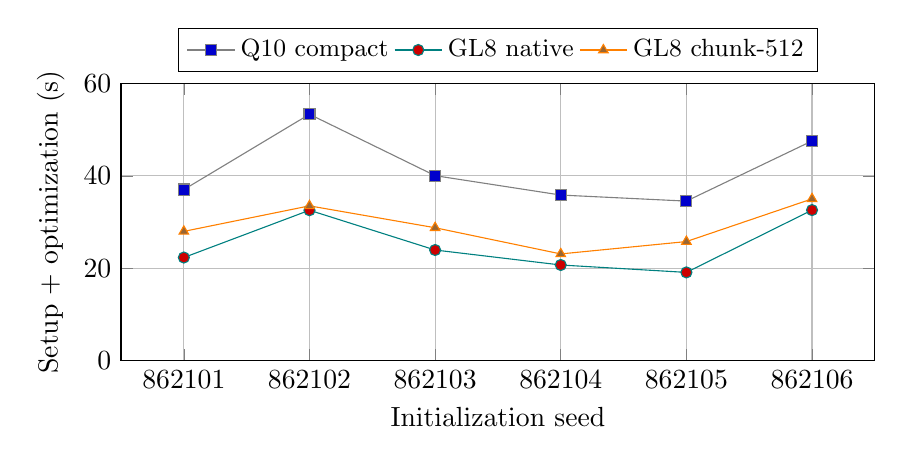
\begin{tikzpicture}\begin{axis}[width=.92\linewidth,height=5.1cm,ymin=0,ymax=60,
xtick={1,2,3,4,5,6},xticklabels={862101,862102,862103,862104,862105,862106},
xlabel={Initialization seed},ylabel={Setup + optimization (s)},grid=major,
legend style={at={(0.5,1.04)},anchor=south,legend columns=3,font=\small}]
\addplot+[mark=square*,color=gray] coordinates {(1,37.011357) (2,53.326424) (3,40.025775) (4,35.828603) (5,34.515535) (6,47.547321)};\addlegendentry{Q10 compact}
\addplot+[mark=*,color=teal] coordinates {(1,22.297896) (2,32.538588) (3,23.922210) (4,20.678393) (5,19.075999) (6,32.572024)};\addlegendentry{GL8 native}
\addplot+[mark=triangle*,color=orange] coordinates {(1,27.961008) (2,33.489470) (3,28.747084) (4,23.076026) (5,25.755669) (6,35.001419)};\addlegendentry{GL8 chunk-512}
\end{axis}\end{tikzpicture}
\caption{Every observed paired solve in the representation campaign. All 18 pass. Connected points identify backends across different initialization seeds; they do not interpolate a continuous experimental variable.}\label{fig:paired-internal}\end{figure}

\subsection{Source-pinned public solves}

\begin{table}[t]
\centering\small
\setlength{\tabcolsep}{4pt}
\caption{Public comparison. Outcomes are accepted/nonconverged/runtime-or-correctness-failure/not-run out of six planned seeds. Time medians in seconds retain all attempted solves. Final column is paired baseline/GL8 setup-plus-optimization geometric mean and number of jointly accepted pairs; values above one favor GL8. NVIDIA arms run in separate windows.}
\label{tab:public}
\begin{tabular}{lcrrrr}\toprule
Method & Outcomes & Opt. s & Setup + opt. s & Process s & Ratio / $n$\\\midrule
FlashNS GL8 & 6/0/0/0 & 23.131 & 23.496 & 25.818 & 1.000 / 6\\
Q10 compact & 6/0/0/0 & 34.090 & 39.248 & 42.877 & 1.658 / 6\\
Collapsed Taylor & 6/0/0/0 & 35.955 & 40.415 & 43.775 & 1.730 / 6\\
Cao ED & 6/0/0/0 & 50.055 & 54.810 & 58.232 & 2.312 / 6\\
Torch coordinate AD & 6/0/0/0 & 64.800 & 70.682 & 74.447 & 2.994 / 6\\
STDE exact (2D) & 6/0/0/0 & 75.376 & 78.650 & 81.400 & 3.368 / 6\\
PhysicsNeMo & 6/0/0/0 & 54.479 & 72.506 & 77.286 & 3.108 / 6\\
cuDNN convolution AD & 6/0/0/0 & 523.492 & 531.241 & 534.903 & 22.865 / 6\\
cuEquivariance polynomial & 6/0/0/0 & 32.155 & 35.729 & 38.697 & 1.555 / 6\\
\bottomrule\end{tabular}
\end{table}


The public matrix plans 54 cells and records 54 actual formal child attempts, of which 54 pass every acceptance criterion. The priority paper group records 36 of 36 planned attempts. All observed formal initial parameter hashes match the corresponding seeds in the original representation campaign; the six planned initializations are reused across experiments, not additional independent seeds for each backend.

Paired baseline/GL8 setup-plus-optimization ratios are Collapsed Taylor: 1.730$\times$ (6 accepted pairs, range 1.482--1.906); Cao ED: 2.312$\times$ (6 accepted pairs, range 2.024--2.607); STDE exact (2D): 3.368$\times$ (6 accepted pairs, range 2.833--3.862); Torch coordinate AD: 2.994$\times$ (6 accepted pairs, range 2.712--3.259). They describe the matched adaptations and common optimizer pipeline. They are not the original papers' speedup claims.

\begin{figure}[t]\centering
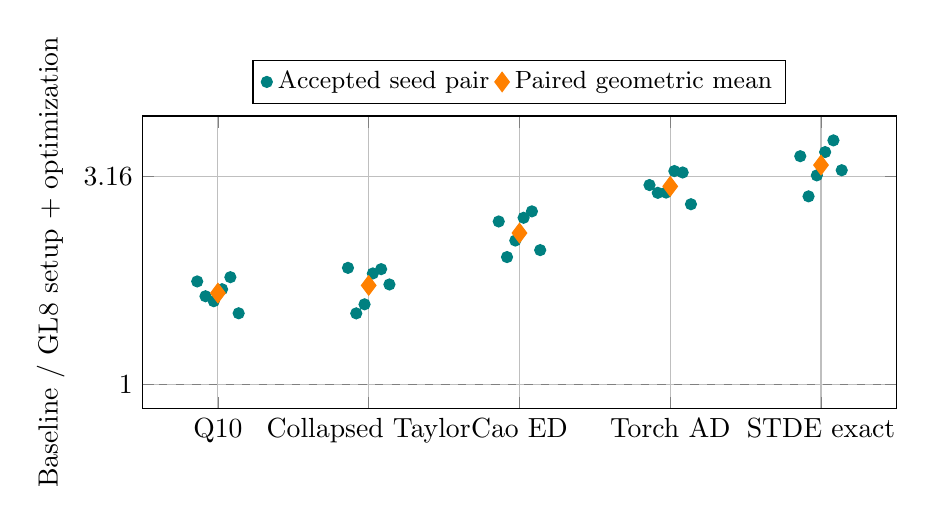
\begin{tikzpicture}\begin{axis}[width=.92\linewidth,height=5.3cm,
xmin=.5,xmax=5.5,ymode=log,log ticks with fixed point,
xtick={1,2,3,4,5},xticklabels={Q10,Collapsed Taylor,Cao ED,Torch AD,STDE exact},
ylabel={Baseline / GL8 setup + optimization},grid=major,
legend style={at={(0.5,1.04)},anchor=south,legend columns=2,font=\small}]
\addplot[gray,dashed,forget plot] coordinates {(.5,1) (5.5,1)};
\addplot[only marks,mark=*,mark size=2pt,teal] coordinates {(0.8625,1.7685157) (0.9175,1.6292653) (0.9725,1.5851020) (1.0275,1.6935076) (1.0825,1.8106506) (1.1375,1.4825818) (1.8625,1.9064955) (1.9175,1.4817714) (1.9725,1.5580050) (2.0275,1.8483542) (2.0825,1.8930807) (2.1375,1.7390763) (2.8625,2.4648008) (2.9175,2.0238531) (2.9725,2.2179618) (3.0275,2.5158157) (3.0825,2.6066059) (3.1375,2.1033487) (3.8625,3.0155709) (3.9175,2.8884972) (3.9725,2.8921820) (4.0275,3.2589793) (4.0825,3.2329917) (4.1375,2.7119036) (4.8625,3.5381748) (4.9175,2.8325723) (4.9725,3.1815392) (5.0275,3.6198600) (5.0825,3.8620535) (5.1375,3.2737326)};\addlegendentry{Accepted seed pair}
\addplot[only marks,mark=diamond*,mark size=3.5pt,orange] coordinates {(1,1.6578672) (2,1.7297226) (3,2.3116925) (4,2.9936746) (5,3.3678945)};\addlegendentry{Paired geometric mean}
\end{axis}\end{tikzpicture}
\caption{Paper-group solve ratios for every jointly accepted initialization pair. Above one favors GL8; the dashed line is equal time. Horizontal offsets separate seed observations, not additional experimental conditions. Table~\ref{tab:public} retains all attempted outcomes and the accepted-pair denominators.}\label{fig:paired-public}\end{figure}

\begin{table}[t]
\centering\small
\setlength{\tabcolsep}{4pt}
\caption{Largest final error over all accepted seeds and both validators, rounded to four decimals. Acceptance uses the unrounded values and every criterion; $n$ is the number of accepted seeds. Unsupported or unattempted methods have no final-error statistic.}
\label{tab:validation}
\begin{tabular}{lrrrrrrr}\toprule
Method & $n$ & PDE & Boundary & Outlet & $u$ & $v$ & $p$\\\midrule
FlashNS GL8 & 6 & 0.0138 & 0.0093 & 0.0025 & 0.0095 & 0.0200 & 0.0099\\
Q10 compact & 6 & 0.0147 & 0.0096 & 0.0024 & 0.0096 & 0.0199 & 0.0109\\
Collapsed Taylor & 6 & 0.0132 & 0.0096 & 0.0025 & 0.0093 & 0.0200 & 0.0091\\
Cao ED & 6 & 0.0136 & 0.0095 & 0.0026 & 0.0091 & 0.0200 & 0.0103\\
Torch coordinate AD & 6 & 0.0146 & 0.0099 & 0.0028 & 0.0097 & 0.0199 & 0.0102\\
STDE exact (2D) & 6 & 0.0141 & 0.0097 & 0.0030 & 0.0094 & 0.0200 & 0.0096\\
PhysicsNeMo & 6 & 0.0146 & 0.0095 & 0.0021 & 0.0096 & 0.0199 & 0.0097\\
cuDNN convolution AD & 6 & 0.0157 & 0.0100 & 0.0023 & 0.0093 & 0.0200 & 0.0112\\
cuEquivariance polynomial & 6 & 0.0150 & 0.0098 & 0.0024 & 0.0094 & 0.0199 & 0.0097\\
\bottomrule\end{tabular}
\end{table}


The nvidia qualification retains 4 failed execution variants. Their complete tracebacks and process costs are in the raw artifact. Formal cells with no passing variant remain not-run; no failed backend is renamed or replaced by the scalar diagnostic.

Qualification process-wall costs, including unsuccessful variants and the original author recipe where applicable, are nvidia 137.927 s, papers 263.687 s. These costs are separate from warm-dependency formal solve timings.

\subsection{Memory and replay tradeoff}

\begin{table}[t]
\centering\small
\setlength{\tabcolsep}{4pt}
\caption{Earlier independent-process replay/memory study: five processes per shape/arm, seven groups of 100 replays per process. Latency is the median of process medians. Allocator measurements are taken before allocating the full-jet correctness oracle; they measure Torch allocation/reservation, not total GPU process memory.}
\label{tab:memory}
\begin{tabular}{rlrrr}\toprule
Interior & Method & Gradient ms & Setup peak MiB & Ready reserved MiB\\\midrule
2,048 & Q10 compact & 3.272 & 87.16 & 102.00\\
2,048 & FlashNS GL8 & 1.578 & 69.61 & 76.00\\
2,048 & GL8 chunk-512 & 2.271 & 42.92 & 56.00\\
16,384 & Q10 compact & 23.539 & 456.72 & 642.00\\
16,384 & FlashNS GL8 & 11.511 & 312.79 & 340.00\\
16,384 & GL8 chunk-512 & 17.908 & 45.88 & 76.00\\
\bottomrule\end{tabular}
\end{table}


At 16,384 interior points, chunk-512 reduces native GL8 setup/capture allocated peak from 312.79 to 45.88 MiB, a reduction of 85.33\%, and ready reserved memory from 340 to 76 MiB. Full-gradient replay increases from 11.511 to 17.908 ms, a 55.58\% cost. At 2,048 points, native GL8 remains the speed-oriented option. No maximum trainable scale or device-traffic reduction is inferred from these counters. A separate 2,048-point native profile attributes 82.30\% of kernel-time sum to library GEMMs; that single-profile share is not a solve-wall attribution.

\subsection{Original author recipe sanity check}

The unmodified Cao NS script naturally completes on the public-comparison GPU. It uses its own six-hidden-layer 64-wide network, FP32 lid-driven-cavity objective and three 1,000-Adam repeats. The archived summary gives AD and ED mean times of 11.132 and 4.613 seconds respectively (ratio 2.413). Its complete-gradient consistency report is retained. This separate reproduction confirms the public script runs; it is not a Kovasznay gPINN solve or a FlashNS comparison.

\section{Three-dimensional transient C36 study}\label{sec:c36}
\subsection{Scientific problem and derivative contract}
This separate manufactured transient incompressible-flow experiment uses
the frozen physical-coordinate source cache and calibration, viscosity
$\nu=0.01$, cutoff width $\eta=1/32$, and the affine/$\tanh$ network
widths 4--128--128--128--128--4. Its outputs represent a three-component
curl potential and pressure, with scales 0.01 and 0.1 respectively. The
prescribed moving-box geometry supplies input features and a compact gate;
the model and particle right-hand side use the learned potential, without
inserting the exact interior velocity. The curl construction enforces
divergence freedom in real arithmetic. Numerical divergence is still
measured rather than assumed to establish all physical acceptance.

For a scalar potential intermediate, the retained raw derivative state is
\begin{equation}
S_{36}(z)=(z,g,H,T,Q,m,n,K),\qquad
Q_{ij}=\partial_{ij}\Delta z,
\label{eq:c36state}
\end{equation}
where $g$, $H$ and $T$ are the spatial gradient, symmetric Hessian and
symmetric third derivative; $m=\partial_t z$, $n=\nabla\partial_t z$ and
$K=\nabla^2\partial_t z$. These blocks have
$1+3+6+10+6+1+3+6=36$ independent channels. They supply the curl velocity,
transient momentum residual and its gradient, including contracted fourth
spatial derivatives of the potential. C36 is a partial-jet contract for
this consumer, not GL8, a full fourth-order jet, or a minimality result.

The canonical objective contains 4,096 interior, 512 initial, 384 boundary
and seven pressure-gauge points. All 4,999 points and all 50,692 parameters
are included. Frozen physical normalization and the original global
family denominators are retained, including during chunk accumulation.
The source and calibration hashes and complete scientific protocol are
identified in the artifact~\cite{flashns3dartifact}. FP64 and disabled TF32
are fixed. This campaign's two original stored initializations are
361901 and 361902; they are not extra H20 formal seeds.

\subsection{Execution changes and numerical qualification}
The H100 packed-gather revision transposes symmetric unpacking through
four cached integer gathers instead of a chain of 54 in-place slice
assignments. It retains the same C36 algebra and local state-autograd
nonlinear pullbacks. Its full-objective GPU proof records 48 comparisons
and 96 saved arrays, covering both original and changed parameters.
The maximum discrepancy is $2.07227\times10^{-5}$ of the unchanged
$10^{-11}+10^{-9}|g_{\rm ref}|$ comparison budget. Its complete native
reference derives from the earlier all-point H100 qualification, which
freshly evaluated native coordinate and parameter AD at every canonical
point; the gather qualification does not rerun that expensive native
reference. Partition agreement alone is not an independent coordinate
oracle.

The subsequent opt-in packed activation computes the six Hessian and
ten third-derivative entries directly, avoiding their full 9- and
27-entry expansion and repacking. A manual analytic transpose reverses
the activation's packed contractions and the actual stable coefficient
program. Gate and curl nonlinear pullbacks still use local state autograd;
this is not a fully manual nonlinear adjoint for the entire model.
For the activation primal $y=\tanh z$ and $e=\exp(-2|z|)$, the frozen
coefficient convention is
\begin{align}
a_1&=4e/(1+e)^2,\qquad a_2=-2ya_1,\\
a_3&=4y^2a_1-2a_1^2,\qquad
a_4=16ya_1^2-8y^3a_1.
\label{eq:stablec36}
\end{align}
The transpose differentiates these evaluated operations, including the
rounded $\tanh$ derivative and the exponential tail, rather than
substituting an idealized fifth derivative at saturated values. Regression
checks include values 0, $\pm10^{-16}$, $\pm10^{-12}$, $\pm20$ and
$\pm40$, with cotangents scaled to $10^8$.

Full canonical CPU qualification at original and changed parameters
records 42 comparisons and 84 preserved arrays for the compiled analytic
variant. A fresh NumPy-only reader passes every comparison; its maximum
error is $9.17612\times10^{-6}$ of the original budget. This rechecks the
preserved H100 native reference ancestry rather than freshly running
native coordinate AD on all CPU points. Exact initial tensor bytes come
from the original checkpoints: regeneration under the newer Torch version
was rejected after 1,804 of 50,692 entries differed by one ULP. That failed
attempt is retained. No tolerance or scientific data was changed. Ten
CPU regression checks pass. These facts do not qualify this new variant's
CUDA execution, CUDA Graph replay, training or physical acceptance.

\subsection{Paired complete-objective performance}
Each reported ratio is the geometric mean of matched baseline/candidate
mean evaluation times. Two frozen initializations each have five
alternating AB/BA pairs, for ten pairs per comparison. Candidate and
C36 parameter-AD windows last at least 60 seconds and contain at least
three complete evaluations. Setup, compilation, warm-up and graph
capture are excluded from these ratios and reported separately. CUDA
timings synchronize each complete evaluation. The native-coordinate-AD
leg has its original special rule of one complete native evaluation per
window. The 95\% intervals use 10,000 paired bootstrap resamples with
seed 795912; they describe these timing pairs, not uncertainty across
PDEs, datasets, hardware or independent training seeds.

\begin{table}[htbp]\centering\small
\setlength{\tabcolsep}{4pt}
\caption{Complete C36 objective and all-parameter-gradient timing against the internal C36 parameter-AD control. Times are means over paired windows in seconds; the ratio is a paired geometric mean, not the ratio of these time means. Ten pairs per row. The first two H100 rows retain the earlier packed-gather source and dense activation. The H100 packed-graph row uses a later packed activation with analytic activation transpose and the same eager packed forward in its parameter-AD control; both arms replay graphs. The final H100 row and the CPU row compile the packed activation in both forward arms and the candidate activation transpose. These different versions and devices are not pooled.}
\label{tab:c36performance}
\begin{tabular}{lrrrr}\toprule
Device / mode & Candidate s & AD s & Ratio & 95\% interval\\\midrule
H100 eager & 1.739582 & 1.692531 & 0.972935 & 0.970474--0.975924\\
H100 graph & 0.484235 & 0.469551 & 0.969678 & 0.969317--0.970075\\
H100 packed graph & 0.328305 & 0.342941 & 1.044582 & 1.044130--1.045051\\
H100 compiled graph & 0.164484 & 0.217771 & 1.323962 & 1.323087--1.324762\\
CPU compiled & 1.865900 & 2.352072 & 1.265086 & 1.203149--1.327900
\\\bottomrule\end{tabular}
\end{table}
The H100 source \texttt{ae51ca643280} remains 2.782\% slower in eager
mode and 3.127\% slower when both arms replay CUDA Graphs. The parameter-AD
control shares C36 forward algebra and is a strong execution baseline;
it is not an independent coordinate derivative oracle or the public
collapsed Taylor library used in the H20 campaign. GPU timing and saved
gradient readers complete naturally with exit zero.

The later H100 packed-graph experiment records 78 comparisons and 156
saved arrays, including both original and changed parameters for both
seeds, direct calls and graph replay, and the original 128/64-point
candidate partitions. The preserved complete native anchors are checked
without a fresh native coordinate-AD rerun. Both remote and local
NumPy-only readers pass all 78 comparisons and reconstruct every timing
window. The maximum numerical error is $2.35186\times10^{-6}$ of the
unchanged comparison budget. Candidate/control window means are
0.328305/0.342941 seconds; the paired ratio is 1.044582, with interval
1.044130--1.045051. This is a 4.458\% throughput improvement against this
matched packed-forward parameter-AD control, with setup, warm-up and
capture outside the timing windows. It is not a pooled comparison with
the older dense-activation experiment, and no new optimizer or physical
acceptance result is inferred. Both workers exit zero; all 106 members
of the complete 161,241,343-byte archive are verified on cluster storage
and locally, and the original GPU lock is released.

An initial compiled CUDA attempt retains 18 passing direct full-gradient
checks but stops before compiled evaluation because Triton is unavailable.
The whole attempt remains failed, with its logs, arrays and complete archive
retained. The successful packed-graph experiment explicitly selects eager
activation plus CUDA Graph replay; it does not silently fall back from
compiler failure. The compiled GPU path is a separate experiment.

The completed compiled H100 experiment uses Torch 2.4.0a0, Triton 3.0.0
and the same frozen scientific data, original stored parameters and timing
protocol. Both arms compile the same packed activation forward; the
candidate also compiles its analytic activation transpose. The old cluster
Torch runtime supplies compiler targets as tuples. An explicit per-process
adapter changes only that representation to Triton's device target, checking
the backend, architecture and warp size against the actual CUDA device.
Kernel source, FP64 dtype and compiler options remain unchanged, and both
arms use the same adapter. No installed Torch or Triton source is modified.

The full canonical compiled check passes 78 comparisons and preserves 156
arrays. Both remote and local NumPy readers pass every comparison, all 20
timing windows and the ten-pair bootstrap reconstruction; maximum error is
$2.35186\times10^{-6}$ of the original numerical budget. Candidate/control
means are 0.164484/0.217771 seconds, with paired ratio 1.323962 and interval
1.323087--1.324762. Compilation, warm-up and graph capture are measured
outside these windows. The complete 161,322,508-byte archive and all 114
members are independently verified on cluster storage and locally. All
owned children finish and the original GPU lock is released. The earlier
compiler failures remain failed, fully archived outcomes; the result does
not imply new training convergence, physical acceptance or solve timing.

The newer CPU variant uses Torch 2.14.1, NumPy 2.5.4, CPU Inductor and
one Torch thread. Both arms compile the same packed forward; only the
candidate supplies the analytic activation transpose. A fresh NumPy-only
reader checks 24 saved gradient arrays, 12 gradient comparisons and all
20 paired timing windows. All checks pass at the original budget. The
1.265$\times$ result is CPU objective-gradient throughput. The H100 compiled
experiment is reported separately above; neither result establishes an
accepted three-dimensional solve.

A separate older source, \texttt{73baa3b281fb}, measures native
coordinate AD with its original recursive derivative cache. Mean
candidate/native times are 2.777272/3,484.283522 seconds, with paired ratio
1,254.839 and interval 1,211.337--1,291.263 (ten pairs). That candidate
predates packed gather, and the baseline predates the later cache-lifetime
repair. The large ratio is specific to that slow recursive native path;
it is not a speedup against the optimized parameter-AD control, the repaired
native implementation or a complete accepted solver. The timing worker,
reader and timing driver exit zero. The original whole controller exits
one due to its earlier failed training stage, which remains a failed
controller outcome rather than being relabeled successful.

\subsection{Frozen-budget training outcomes}
Both H100 engines start from their original fresh initializations and
execute 4,000 Adam updates plus 20 strong-Wolfe L-BFGS calls per seed.
Adam has initial learning rate $10^{-3}$, halved every 1,000 updates,
betas (0.9,0.999) and epsilon $10^{-8}$. L-BFGS uses learning rate one,
history 20, at most 20 iterations and nominal 25 evaluations per call,
zero gradient/change stopping tolerances and a 520-closure cap per seed.
The complete-gradient checks run at frozen Adam checkpoints and after
every L-BFGS call. Each engine passes all 48 scheduled saved-gradient
comparisons. Successful execution and gradient checks do not establish
convergence: the original joint gate requires loss at most $10^{-4}$
and gradient infinity norm at most $10^{-3}$.

\begin{table}[htbp]\centering\small
\setlength{\tabcolsep}{4pt}
\caption{All four C36 training attempts finish the original finite budget. Actual L-BFGS closure counts, final loss and full-gradient infinity norm are shown. Every attempt fails the joint convergence gate; no additional optimizer budget is silently appended.}
\label{tab:c36training}
\begin{tabular}{lrrrrl}\toprule
Engine & Seed & Closures & Loss & $\|g\|_\infty$ & Gate\\\midrule
Explicit & 361901 & 444 & 0.00054021 & 0.00075071 & Fail\\
Explicit & 361902 & 438 & 0.00051678 & 0.00128521 & Fail\\
Parameter AD & 361901 & 449 & 0.00053870 & 0.00059044 & Fail\\
Parameter AD & 361902 & 443 & 0.00051532 & 0.00206306 & Fail
\\\bottomrule\end{tabular}
\end{table}
All four losses remain above $10^{-4}$. The explicit seed 361902 and
parameter-AD seed 361902 also exceed the gradient limit. The evaluated
training sources are \texttt{7281faed9ec4} (explicit) and
\texttt{de1d223} (parameter AD); they do not train the later CPU analytic
activation variant. No accepted three-dimensional time-to-accuracy or
whole-solver acceleration is available.

\subsection{Independent physical observations and failures}
The unchanged holdout seed 794701 supplies 4,096 stratified and 4,096
uniform-volume points, seven time slices with 256 points each, 512 initial
points, 384 boundary points and seven pressure-gauge points. Native
coordinate AD observes the final learned model on H100; NumPy reconstructs
the physical metrics. Learned-velocity trajectories use SciPy DOP853 for
27 particles at 129 uniform output times plus the critical times. Both
original refinements complete: $(\mathrm{rtol},\mathrm{atol},\mathrm{max\ step})$
are $(10^{-9},10^{-11},1/64)$ and $(10^{-11},10^{-13},1/128)$.
The exact velocity is used for error comparison, never as the trajectory
right-hand side. Both stratified and uniform field gates and the trajectory
gate must pass; time-slice and regional reports remain diagnostics.

\begin{table}[htbp]\centering\small
\setlength{\tabcolsep}{4pt}
\caption{C36 final field failures. S/U denote stratified/uniform holdouts. Velocity errors are relative L2; momentum and corrected pressure use the original physical normalization. Row limits are velocity 0.01, momentum 0.01 and pressure 0.001. All displayed values exceed their corresponding gate; complete region and time-slice values remain in the result JSON.}
\label{tab:c36fields}
\begin{tabular}{lrrrrrr}\toprule
Engine & Seed & Vel. S & Vel. U & Mom. S & Press. S & Press. U\\\midrule
Explicit & 361901 & 0.020528 & 0.043743 & 0.014220 & 0.025935 & 0.003022\\
Explicit & 361902 & 0.018808 & 0.034605 & 0.013856 & 0.022480 & 0.003407\\
Parameter AD & 361901 & 0.020331 & 0.043126 & 0.014276 & 0.024746 & 0.002837\\
Parameter AD & 361902 & 0.018497 & 0.034154 & 0.013832 & 0.019825 & 0.003094
\\\bottomrule\end{tabular}
\end{table}
\begin{table}[htbp]\centering\small
\setlength{\tabcolsep}{4pt}
\caption{C36 trajectories from the stricter original DOP853 refinement. Endpoint error must be at most 0.001; refinement change must be at most $10^{-7}$. All refinement tests pass but all endpoint tests fail, so no row passes physical acceptance.}
\label{tab:c36trajectories}
\begin{tabular}{lrrrl}\toprule
Engine & Seed & Endpoint & Refinement change & Gate\\\midrule
Explicit & 361901 & 0.023166 & $7.2297\times10^{-11}$ & Fail\\
Explicit & 361902 & 0.029803 & $7.2587\times10^{-11}$ & Fail\\
Parameter AD & 361901 & 0.022762 & $7.2325\times10^{-11}$ & Fail\\
Parameter AD & 361902 & 0.029980 & $7.1729\times10^{-11}$ & Fail
\\\bottomrule\end{tabular}
\end{table}
For all four checkpoints, initial/boundary velocity and gauge errors are
exactly zero. Stratified normalized divergence remains at most
$2.01\times10^{-14}$, and divergence-gradient RMS at most
$3.05\times10^{-12}$; their limits are $10^{-3}$ and 0.02. Momentum-gradient
RMS also passes its 0.02 limit. These satisfied gates coexist with failed
velocity, stratified momentum, corrected-pressure and trajectory-endpoint
criteria. Accurate divergence and tightly converged ODE integration do not
establish an accurate learned velocity field.

The observer source \texttt{1f1983a2b015} repairs a recursive native
derivative closure cycle that retained CUDA graphs until garbage collection.
The unchanged checkpoints and physical protocol then complete; the earlier
OOM and its raw logs remain archived. The repair preserves derivative order
and parameter dependence. It is checked against original native states and
all 50,692 gradient entries at two points; sixteen repeated native
observations keep allocated CUDA memory constant at 67,514,880 bytes.
This limited memory qualification supplies no repaired-native paired
performance result.

Each checkpoint's remote and local NumPy readers pass 117 saved-array
checks. They verify hashes, loss/gradient anchors, field residual metrics,
trajectory error summaries and refinement statistics. They do not rerun
the optimizer trajectory or independently reintegrate the ODE. The reader
checks analytic forcing at its original tolerance and retains sealed
source bytes for cancellation-sensitive residual subtraction; a prior
cross-version rounding failure is preserved and no tolerance is widened.

\subsection{Evidence and current limits}
The public machine-readable results preserve every timing pair, all
four training outcomes, and all final physical observations, with full
source/protocol/raw-array hashes~\cite{flashns3dartifact}. GPU timing and
physical archives have fully verified cluster and local copies; the
complete training histories have verified cluster archives, while smaller
training anchors are also available locally. The complete new CPU packet
is verified locally only. Publication of compact result JSON files is
not publication of every raw checkpoint or profiler trace.

The unmodified source cache and calibration remain frozen. Neither
optimization budgets, physical limits, accepted seeds nor global loss
denominators are weakened in response to these failures. The analytic activation remains an opt-in research path: its eager CUDA
Graph and compiled CUDA Graph variants now have full-objective qualification
and paired H100 timings. Trained accuracy and accepted solve timing remain
open work; neither the CPU nor the H100 throughput ratio
implies three-dimensional physical acceptance.


\section{Discussion and limits}
The derivative consumer offers an execution opportunity even after replacing
nested coordinate AD with Taylor-mode computation. GL8 removes independent
third-order information that the fixed diffusion-gradient consumer never
reads, while preserving lower derivatives required by nonlinear convection.
Its explicit transpose is part of the optimization program, not an
afterthought to a forward-only operator. The measured effect nevertheless
combines representation, pointwise kernels, graph scheduling and parameter
backward; the native-versus-compiled-Q10 solve comparison does not isolate a
pure representation effect.

Replay and solve ratios need not match. Optimizer work, line searches and
fixed validation remain outside the accelerated derivative program. Small
floating-point differences can change an L-BFGS trajectory and its closure
count. Setup also differs between compiled public adapters, JAX and explicit
native kernels, even with warmed dependency caches. We therefore report
every timing scope and actual iteration/evaluation count rather than
extrapolating a replay factor to the whole training run.

Chunking addresses a different engineering constraint. It bounds the
intermediate execution workspace and permits a substantial allocator
reduction at the measured larger shape, while paying for input copies,
extra replay launches and gradient accumulation. The fixed data and
optimizer remain resident. We measured neither an OOM boundary nor the
maximum trainable point count, and do not infer those from the two tested
shapes. Torch allocator counters cannot rank total process memory against
JAX's allocator.

The external comparisons must be read within their adaptations. ED and
collapsed Taylor supply public second-order operators extended to a
third-order gradient-enhanced consumer; this is not their original training
benchmark. Exact two-coordinate STDE preserves a deterministic target but
does not test stochastic amortization in high dimensions. The unmodified
cuEquivariance polynomial arm has an all-points Q10 boundary policy, unlike
the compact interior/value-only policy of the paper adapters. Its timing
therefore reflects both a library implementation and that inherited policy.
These differences are recorded rather than erased by a common name.

The representation campaign's six initializations provide a paired view of
one fixed-data manufactured PDE. The public comparison reports its actual
completed-seed coverage separately. These initializations do not measure
variation across PDEs, sampled datasets, network
families or hardware. Repeated replay groups within a qualification process
are timing observations, not additional independent training seeds. The
prior representation study's independent processes are kept separate from
the public qualification process. No speed claim in this paper is extended
to stochastic STDE++ constructions, variable viscosity, nonlinear coordinate
maps, sample-coupled layers, second parameter derivatives or nonlocal losses.

The new three-dimensional transient case adds full-objective derivative
qualification, paired execution measurements and complete failed physical
observations. It has not established an accepted three-dimensional solve.
A stronger general-purpose evaluation would add a second nonlinear PDE,
accepted transient solutions, variable-coefficient operators and a broader
activation/network family. It would also compare cold start and
native framework optimizers, measure actual device traffic and examine
generalized consumer selection. These remain open experiments rather than
implied consequences of the current implementation.

\section{Conclusion}
FlashNS gives a concrete consumer contract for high-order PINN training:
propagate a closed value/gradient/Hessian/gradient-Laplacian state and
transpose every local dependency into the complete parameter gradient.
The H20 experiments evaluate that contract under an unchanged FP64
Navier--Stokes objective and independent numerical acceptance. The compact
native path and its chunked alternative offer distinct speed and workspace
tradeoffs. The original H20 evidence supports that tested solve setting. The earlier
C36 packed-gather study qualifies full derivatives but is slower than its
parameter-AD control, and the completed C36 training budgets fail physical
acceptance. The later CPU analytic activation achieves a paired 1.265$\times$
objective-gradient speedup with an equally compiled forward baseline. The subsequent eager packed activation and analytic activation transpose
provide 1.0446$\times$ matched-forward H100 CUDA Graph throughput. Compiling
the packed forward in both arms and the candidate activation transpose gives
1.3240$\times$ against the equally compiled parameter-AD control. Accepted
three-dimensional solve acceleration remains unestablished; broader scientific claims require further experiments.


\begin{thebibliography}{99}
\bibitem{pinn}
M. Raissi, P. Perdikaris, and G. E. Karniadakis.
Physics-informed neural networks: A deep learning framework for solving forward and inverse problems involving nonlinear partial differential equations.
\emph{Journal of Computational Physics}, 378:686--707, 2019.
\url{https://doi.org/10.1016/j.jcp.2018.10.045}.
\bibitem{gpinn}
Jeremy Yu, Lu Lu, Xuhui Meng, and George Em Karniadakis.
Gradient-enhanced physics-informed neural networks for forward and inverse PDE problems.
arXiv:2111.02801, 2021.
\url{https://arxiv.org/abs/2111.02801}.
\bibitem{cao}
Wenbo Cao, Zhe Lu, and Weiwei Zhang.
Verified residual-specific explicit derivative kernels for physics-informed learning and discretized PDE adjoints.
arXiv:2606.29702, 2026.
\url{https://arxiv.org/abs/2606.29702}.
\bibitem{cmtad}
Felix Dangel, Tim Siebert, Marius Zeinhofer, and Andrea Walther.
Collapsing Taylor Mode Automatic Differentiation.
\emph{Advances in Neural Information Processing Systems}, 38, 2025.
\url{https://papers.nips.cc/paper_files/paper/2025/hash/d835e25415cfe4d6d48a0be3b7b763bb-Abstract-Conference.html}.
\bibitem{stdepp}
Zekun Shi, Zheyuan Hu, Min Lin, and Kenji Kawaguchi.
STDE++: Polynomial-Time Amortization for Linear Differential Operators.
\emph{Journal of Machine Learning Research}, 27(114):1--50, 2026.
\url{https://www.jmlr.org/papers/v27/25-1474.html}.
\bibitem{stde}
Zekun Shi, Zheyuan Hu, Min Lin, and Kenji Kawaguchi.
Stochastic Taylor Derivative Estimator: Efficient amortization for arbitrary differential operators.
\emph{Advances in Neural Information Processing Systems}, 37, 2024.
\url{https://proceedings.neurips.cc/paper_files/paper/2024/hash/dd2eb5250696753ea37141bbd89bb569-Abstract-Conference.html}.
\bibitem{stdecode}
sail-sg. STDE official public implementation.
Source commit \texttt{fae88663b1d2f1b0666d4d250c38a3c34b852ac0}.
\url{https://github.com/sail-sg/stde}.
\bibitem{physicsnemo}
NVIDIA. PhysicsNeMo public implementation.
Source commit \texttt{b45a5c810c741e6b41f8515be24c51121f8fc21f}.
\url{https://github.com/NVIDIA/physicsnemo}.
\bibitem{cudnn}
NVIDIA. CUDA Deep Neural Network library (cuDNN).
\url{https://developer.nvidia.com/cuda/cuda-x-libraries/cudnn}.
\bibitem{cueq}
NVIDIA. cuEquivariance public implementation.
Source commit \texttt{70674ada7a00372e88ebe99969c700a6dcddd08f}.
\url{https://github.com/NVIDIA/cuEquivariance}.
\bibitem{flashns3dartifact}
Dezhen Lu. FlashNS C36 experiment and reproducibility artifact.
Evidence snapshot \texttt{37ced2805131fcfaba6f7f89f8b0b1d17e5cef28},
October 13, 2026; per-experiment runtime hashes are retained in the result files.
\href{https://github.com/0z5a/FlashNS/tree/37ced2805131fcfaba6f7f89f8b0b1d17e5cef28/research/c36-potential-proof}{Public C36 source, frozen protocols and result JSON files}.
\end{thebibliography}


\appendix

\section{Explicit local transpose}
For completeness, let $\bar y$, $\bar g_y$, $B_y$ and $\bar t_y$ denote
output adjoints. Here $B_y$ is symmetric and represents the Frobenius
pairing with the full symmetric Hessian. If the stored off-diagonal
Hessian channel has adjoint $\beta_{12}$, this convention sets
$(B_y)_{12}=(B_y)_{21}=\beta_{12}/2$. Define $h=\operatorname{tr}H$,
$c=g^\top g$ and $Q=gh+2Hg$. Transposing the local differential gives
\begin{align}
\bar t&=a_1\bar t_y,\\
\bar H&=a_1 B_y+a_2\big((\bar t_y^\top g)I+
                 \bar t_y g^\top+g\bar t_y^\top\big),\\
\bar g&=a_1\bar g_y+2a_2B_y g
          +a_2(h\bar t_y+2H\bar t_y)
          +a_3(c\bar t_y+2g(g^\top\bar t_y)),\\
\bar z&=a_1\bar y+a_2\bar g_y^\top g
          +\langle B_y,a_2H+a_3gg^\top\rangle_F
          +\bar t_y^\top(a_2t+a_3Q+a_4gc).
\end{align}
The packed input Hessian adjoint is obtained by transposing symmetric
unpacking: diagonal entries are unchanged and each off-diagonal channel
receives the sum of its two matrix entries. This convention prevents a
factor-of-two error. All terms contribute to the shared parameter VJP
through the affine transpose; no activation derivative order is discarded
because it exceeds the forward coordinate order.

The argument assumes fixed physical coordinates, coordinate-independent
affine parameters, a fixed contraction and sufficiently smooth pointwise
activations. Let $P$ map a complete third-order raw jet to $(z,g,H,t)$.
The chain rule establishes $P F_{\rm full}=F_{\rm GL8}P$ for each supported
layer. Induction gives the same identity for a supported network. Since
the residual loss factors through $P$, its real-arithmetic parameter
derivative agrees with the full-jet derivative. This is a closure and
transpose argument for a stated consumer; it is not a proof that no other
representation could use fewer channels.

\section{Chunk accumulation and storage contract}
Partition interior and boundary points into finite chunks. With the
original weights, the loss is the sum of chunk contributions and its
parameter gradient is the sum of their parameter gradients. The executor
zeros accumulators once at the beginning of a closure, copies a chunk into
the reusable graph inputs, replays, and accumulates its loss and gradient.
Tail padding has zero weight. Every chunk uses the same parameter version;
the optimizer can update parameters only after the complete closure.

For maximum chunk size $M$, intermediate derivative storage is proportional
to $M$ times the retained layer-channel widths. Fixed point data still grow
with total point count, and parameter/optimizer storage is not bounded by
$M$. The eight-channel contraction removes two hidden coordinate channels;
it does not by itself prove a 20\% reduction in total live memory. At 2,048
interior points, compact logical point/channel rows decrease from
$10(2048)+512=20,992$ to $8(2048)+512=16,896$. Actual allocator measurements
include further temporaries and graph pools.

Captured outputs are borrowed until the next replay. Graph parameter
storage can be updated in place; replacing its storage or using an
incompatible stream/layout is rejected. Comparing a previously returned
borrowed scalar after another closure would compare an overwritten value.
The validation harness checks each live loss/gradient before replay and
checks updated parameter storage separately.



\section{Original H20 source and evidence provenance}
The original two-dimensional H20 execution source is commit
\texttt{286d7e394c8bd39f9aa409715afe9f1bac915cec}, based on public main
\texttt{7c261ea5635cdcec1bf98b72d1105dcf0b486087} and a preserved local
implementation snapshot. The baseline adapters are separate frozen runtime
files. Table~\ref{tab:sources} identifies upstream sources; full tree/blob
hashes, runtime file SHA256 values and all invocation arguments accompany
the artifact. Pinning distinguishes the public collapsed transform from
the project's own compiled full-jet backend.

\begin{table}[h]
\centering\small
\caption{Pinned public baseline sources. Full commit IDs are retained in
the machine-readable source manifests.}\label{tab:sources}
\begin{tabular}{lll}\toprule
Implementation & Public repository & Commit prefix\\\midrule
Cao ED & \href{https://github.com/Cao-WenBo/ExplicitDifferentiation}{Cao-WenBo/ExplicitDifferentiation} & \texttt{a524575baa62}\\
Collapsed Taylor & \href{https://github.com/f-dangel/torch-jet}{f-dangel/torch-jet} & \texttt{2e49005ee4ae}\\
STDE & \href{https://github.com/sail-sg/stde}{sail-sg/stde} & \texttt{fae88663b1d2}\\
PhysicsNeMo & \href{https://github.com/NVIDIA/physicsnemo}{NVIDIA/physicsnemo} & \texttt{b45a5c810c74}\\
cuEquivariance & \href{https://github.com/NVIDIA/cuEquivariance}{NVIDIA/cuEquivariance} & \texttt{70674ada7a00}\\\bottomrule
\end{tabular}
\end{table}

Original JSON reports, progress histories, complete profiler event names,
stdout/stderr, final parameter tensors, protocols and natural process-exit
receipts are preserved. Every archive is copied off the GPU instance and
checked against its recorded whole-archive SHA256 before extraction; every
manifested member is then checked individually. Analysis rejects altered
data, optimizer configurations, unmatched initial parameters, repeated
seed/arm attempts and claimed convergence that violates either validator.
Archive-level verification includes metadata as well as numerical reports.

One inherited optimizer-protocol description still lists the earlier
\texttt{formal\_initialization\_seeds} 75101--75103. That field does not
select parameters in the solver. The frozen campaign seed list, each actual
child's \texttt{--seed} argument and the reported initial tensor-byte hashes
identify the six formal initializations 862101--862106. We preserve the
original metadata bytes and state this discrepancy rather than silently
rewriting the raw reports.

Preparation-only failures are also retained. A local boundary-cardinality
assertion initially counted shared outlet coordinates twice; the frozen
problem always had 512 boundary coordinates, and no numerical data changed.
An earlier archive check correctly rejected an SCP transfer before transfer
completion. Neither event caused a formal training retry or a changed
scientific threshold. GPU comparison uses only the final frozen compact
adapter packet, whose 460 runtime source hashes are checked before each
admitted window.

The initial implementation regression ran 547 CPU checks with two existing
upstream Euler dependency skips and 129 full-width GPU checks. Full-width
Compute Sanitizer memcheck completed 112 checks with zero errors. Small
network racecheck, initcheck and synccheck each completed 60 checks with
zero errors; an earlier full-width racecheck was interrupted for
instrumentation cost and is not counted as completed. These tests establish
stated regression coverage, not correctness for every unsupported consumer.


\section{Every planned public solve}
\small\setlength{\tabcolsep}{4pt}
\begin{longtable}{rllrr}
\caption{All 54 planned public cells, without failed-attempt filtering. Setup plus optimization is in seconds; closure counts are actual. Six paired initialization seeds are reused across methods.}\\
\toprule Seed & Method & Outcome & Setup + opt. & Closures\\\midrule\endfirsthead
\toprule Seed & Method & Outcome & Setup + opt. & Closures\\\midrule\endhead
862101 & FlashNS GL8 & accepted & 21.854 & 6833\\
862102 & FlashNS GL8 & accepted & 32.786 & 9032\\
862103 & FlashNS GL8 & accepted & 25.138 & 7279\\
862104 & FlashNS GL8 & accepted & 21.068 & 6635\\
862105 & FlashNS GL8 & accepted & 18.966 & 6261\\
862106 & FlashNS GL8 & accepted & 30.989 & 8685\\
862101 & Q10 compact & accepted & 38.649 & 6733\\
862102 & Q10 compact & accepted & 53.417 & 9089\\
862103 & Q10 compact & accepted & 39.846 & 7076\\
862104 & Q10 compact & accepted & 35.679 & 6481\\
862105 & Q10 compact & accepted & 34.340 & 6309\\
862106 & Q10 compact & accepted & 45.944 & 8010\\
862101 & Collapsed Taylor & accepted & 41.665 & 7080\\
862102 & Collapsed Taylor & accepted & 48.582 & 8054\\
862103 & Collapsed Taylor & accepted & 39.165 & 6700\\
862104 & Collapsed Taylor & accepted & 38.941 & 6678\\
862105 & Collapsed Taylor & accepted & 35.904 & 6265\\
862106 & Collapsed Taylor & accepted & 53.893 & 8837\\
862101 & Cao ED & accepted & 53.866 & 6788\\
862102 & Cao ED & accepted & 66.355 & 8142\\
862103 & Cao ED & accepted & 55.754 & 6978\\
862104 & Cao ED & accepted & 53.004 & 6559\\
862105 & Cao ED & accepted & 49.436 & 6301\\
862106 & Cao ED & accepted & 65.182 & 8019\\
862101 & Torch coordinate AD & accepted & 65.903 & 6651\\
862102 & Torch coordinate AD & accepted & 94.703 & 9259\\
862103 & Torch coordinate AD & accepted & 72.703 & 7239\\
862104 & Torch coordinate AD & accepted & 68.661 & 6866\\
862105 & Torch coordinate AD & accepted & 61.316 & 6233\\
862106 & Torch coordinate AD & accepted & 84.040 & 8278\\
862101 & STDE exact (2D) & accepted & 77.324 & 6708\\
862102 & STDE exact (2D) & accepted & 92.869 & 7910\\
862103 & STDE exact (2D) & accepted & 79.977 & 6920\\
862104 & STDE exact (2D) & accepted & 76.264 & 6629\\
862105 & STDE exact (2D) & accepted & 73.246 & 6395\\
862106 & STDE exact (2D) & accepted & 101.451 & 8549\\
862101 & PhysicsNeMo & accepted & 73.710 & 6818\\
862102 & PhysicsNeMo & accepted & 93.615 & 8718\\
862103 & PhysicsNeMo & accepted & 60.251 & 6846\\
862104 & PhysicsNeMo & accepted & 70.725 & 6542\\
862105 & PhysicsNeMo & accepted & 71.302 & 6418\\
862106 & PhysicsNeMo & accepted & 95.941 & 8988\\
862101 & cuDNN convolution AD & accepted & 516.349 & 6709\\
862102 & cuDNN convolution AD & accepted & 699.179 & 9049\\
862103 & cuDNN convolution AD & accepted & 546.132 & 7110\\
862104 & cuDNN convolution AD & accepted & 498.826 & 6497\\
862105 & cuDNN convolution AD & accepted & 488.845 & 6367\\
862106 & cuDNN convolution AD & accepted & 662.827 & 8580\\
862101 & cuEquivariance polynomial & accepted & 35.119 & 6654\\
862102 & cuEquivariance polynomial & accepted & 45.720 & 7972\\
862103 & cuEquivariance polynomial & accepted & 36.338 & 6810\\
862104 & cuEquivariance polynomial & accepted & 34.258 & 6482\\
862105 & cuEquivariance polynomial & accepted & 33.449 & 6208\\
862106 & cuEquivariance polynomial & accepted & 47.182 & 8067\\
\bottomrule\end{longtable}\normalsize


\end{document}
